\chapter{\uppercase {Background}}
\label{sec:background}
\begin{figure}[t]
  \centering
  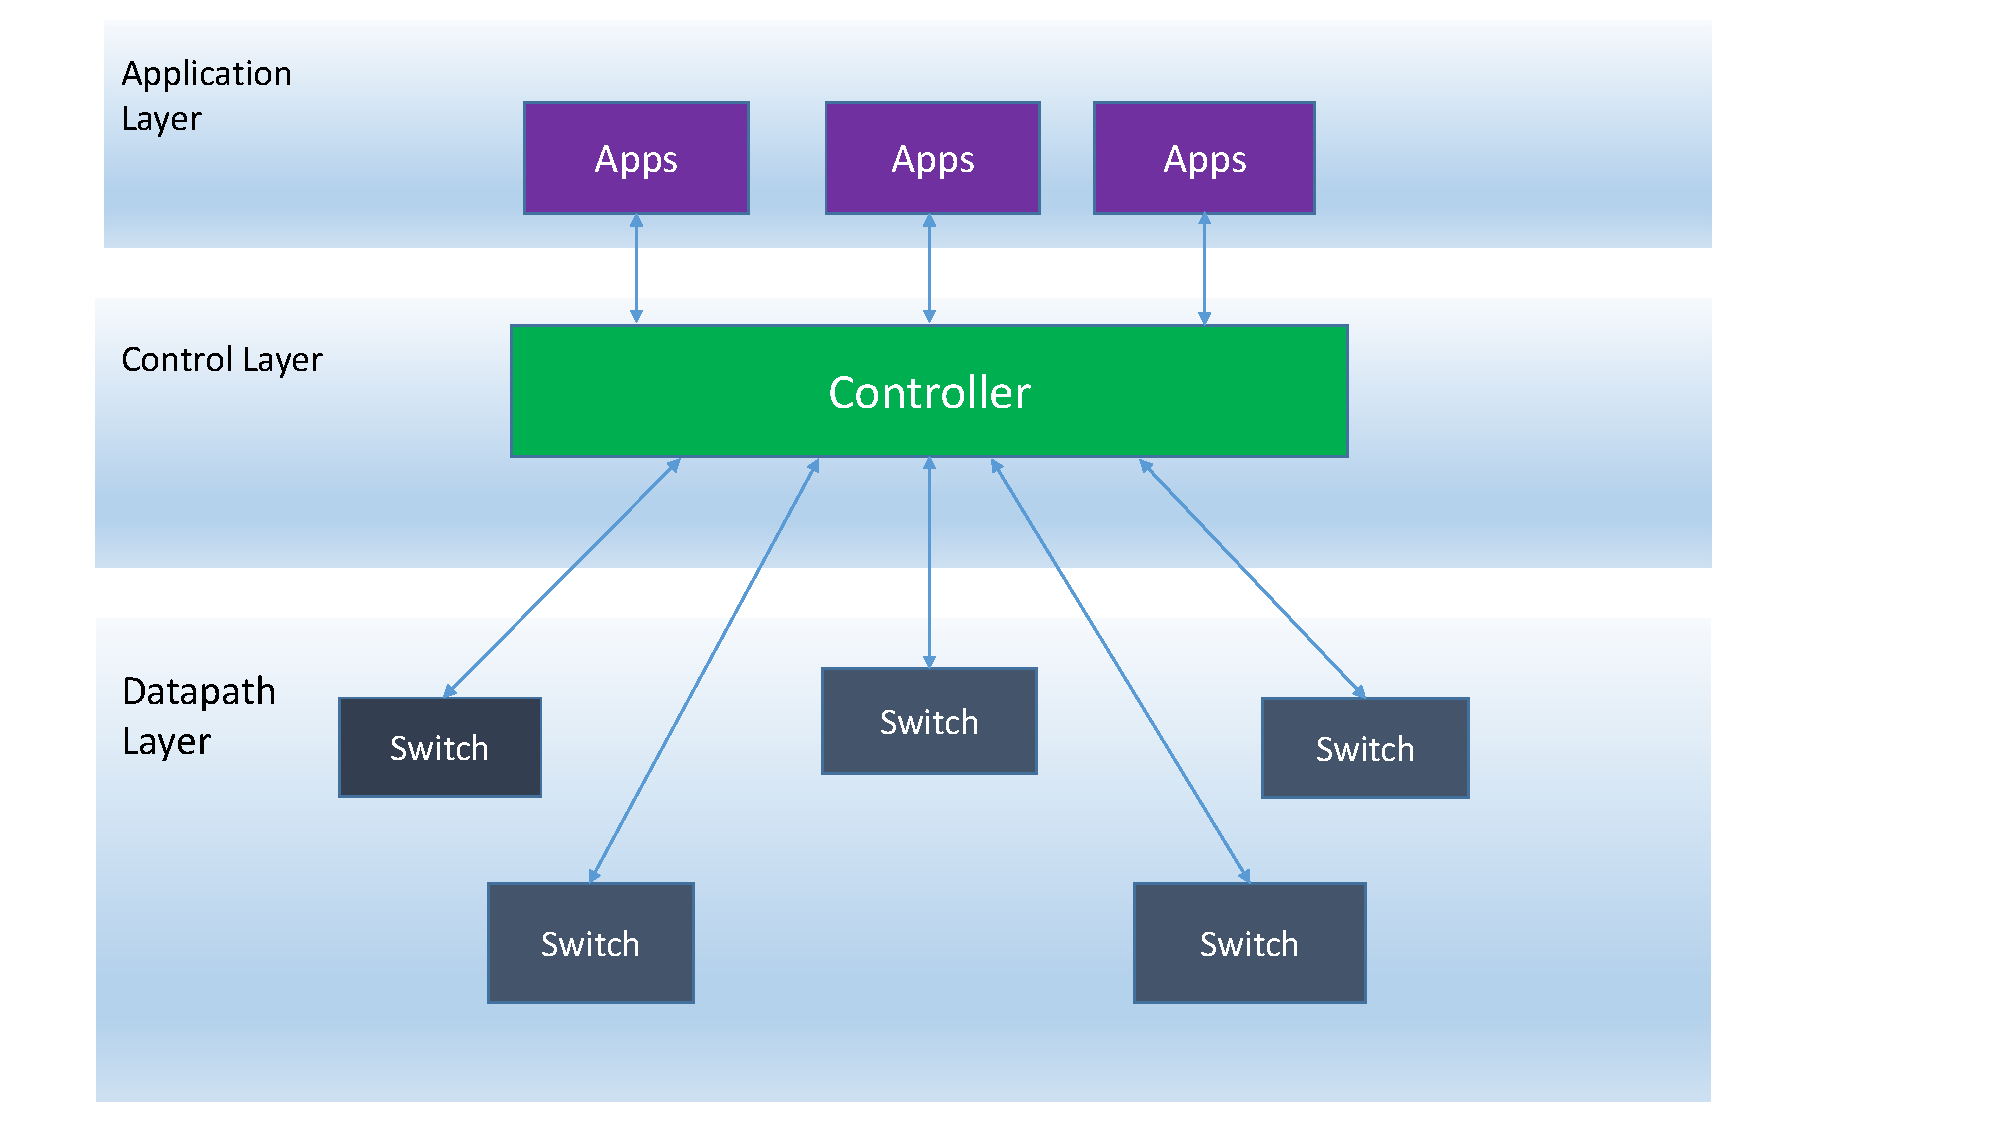
\includegraphics[width=1\textwidth]{figures/SDN.pdf}
  \caption{Overview of Software Defined Networking (SDN) architecture.}
  \label{fig:SDN}
\end{figure}

\section{Software Defined Networking.}
Network reconfigurability is a major challenge in the networking industry. The explosion of mobile devices and cloud services have necessiated the need for on-demand installation of services and reconfiguration of flow rules according to changing traffic patterns. In addition, network elements like routers and switches have their own unique interfaces and as such management of network components is a source of concern for network operators. As network grows, this complexity increases exponentially and rolling out new services becomes a tedious and complicated proces.

Software Defined Networking (SDN) is an architecture which addresses these challenges by decoupling the control and forwarding functions. This enforces abstraction of underlying implementation and enables applications or network services to be developed using the abstractions as shown in Figure~\ref{fig:SDN}. This simple and elegant design also provides applications a centralized view of the network. As a result, it has sparked tremendous research interest in providing a scalable, secure and programmatic approach towards the challenges discussed above. While SDN is a revolutionary approach, it is still mainly geared towards wired networks. The wireless networks have not recieved much attention in this regard. Through \aetherflow, we provide a protocol independent approach for bringing wireless into SDN model. In this thesis, we go a step further and provide a mechanism for dynamic radio resource management to obtain true network visibility in a heterogeneous network.     

\begin{figure}[t]
  \begin{minipage}{\textwidth}
      \centering
      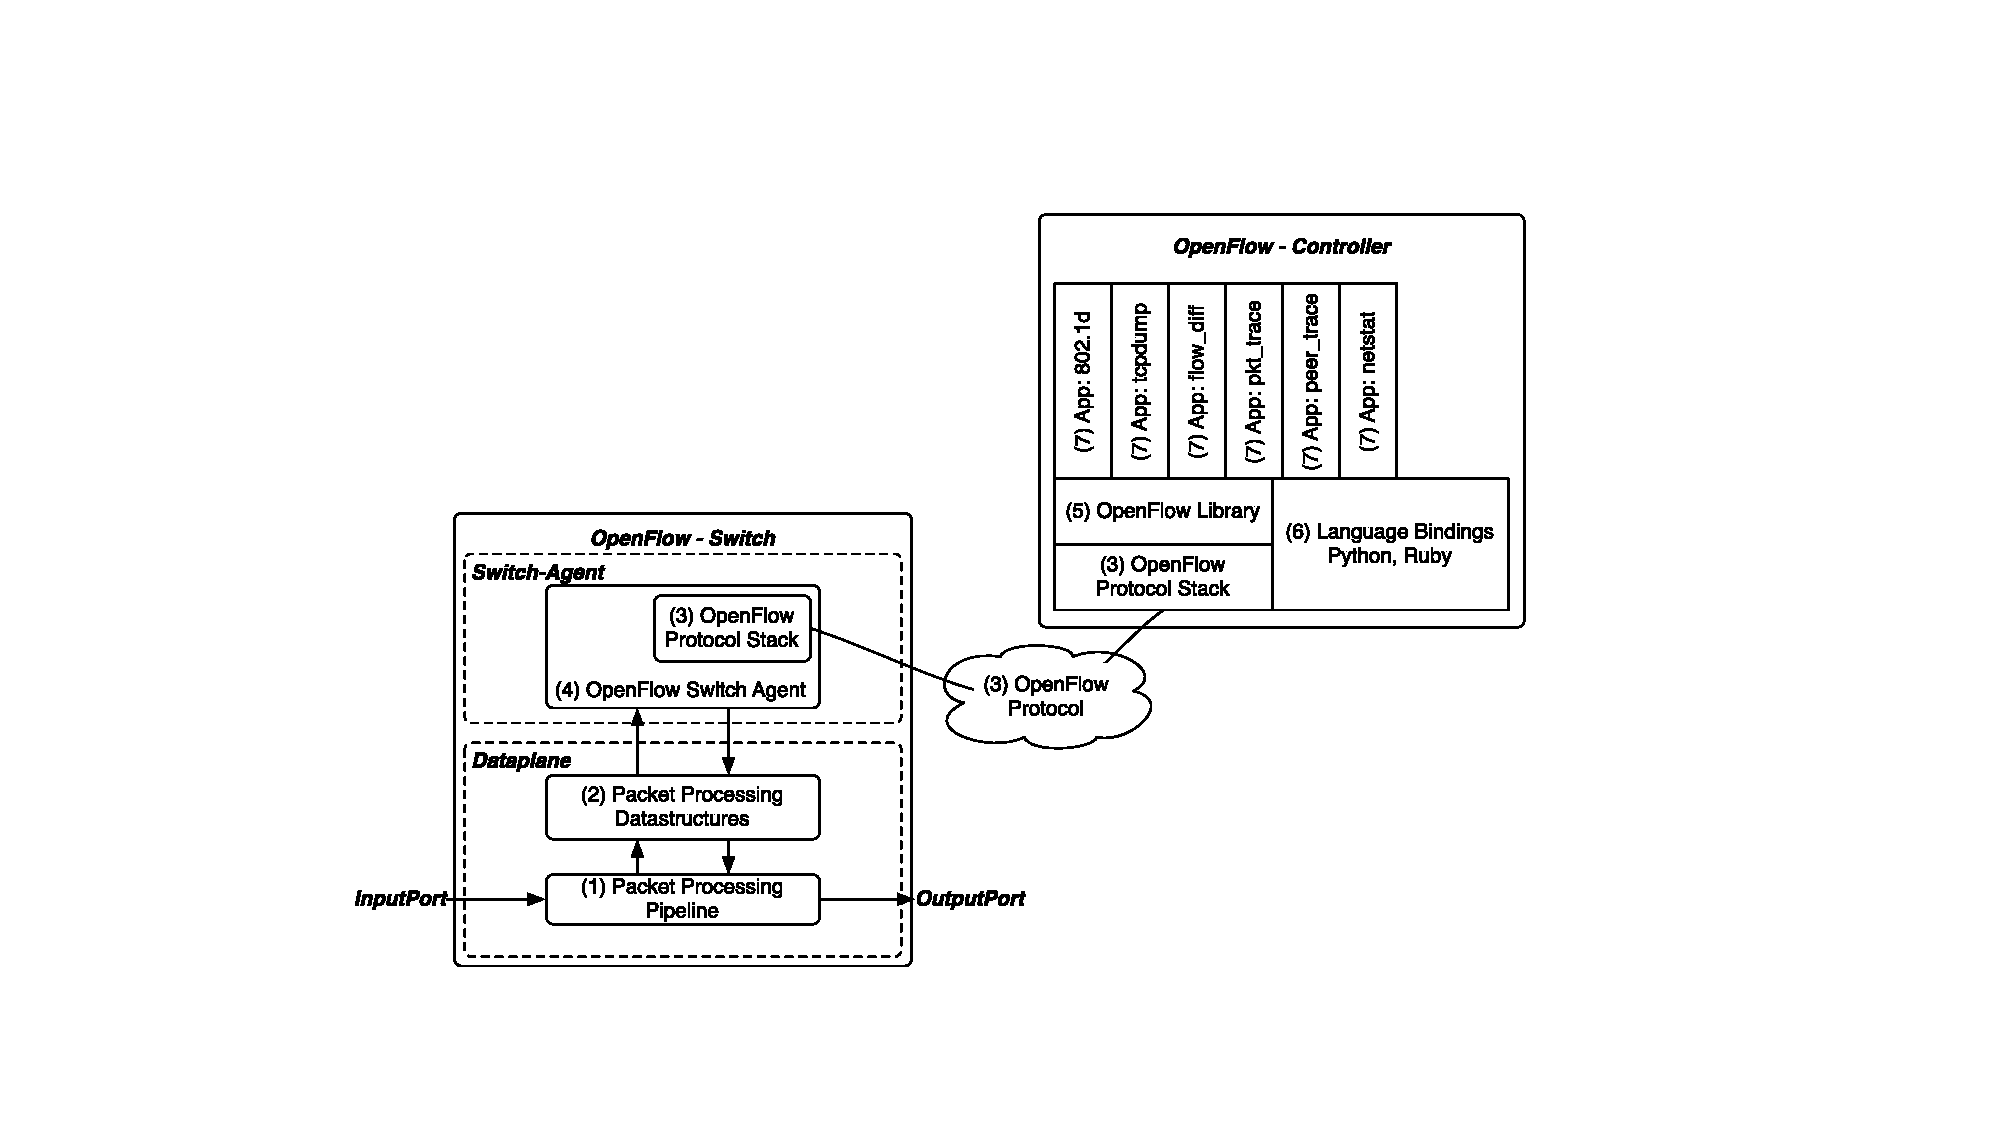
\includegraphics[width=1\textwidth]{figures/OpenFlow.pdf}
      \caption[SDN ecosystem with OpenFlow protocol.]{SDN ecosystem with OpenFlow protocol\protect\footnotemark.}
%  \caption[Caption for LOF]{SDN Ecosystem with OpenFlow protocol\protect\footnotemark}
%      \caption[SDN Ecosystem with OpenFlow protocol]{SDN Ecosystem with OpenFlow protocol\footnote{Courtesy: flowgrammable.org}}
      \label{fig:OpenFlow}
  \end{minipage}  
\end{figure}
\section{OpenFlow.}
OpenFlow is an open standard, that began as research project, which allows researchers to experiment with innovative protocols on network switches, without the requirement of exposure to thier internal implementations. OpenFlow\cite{openflow} builds upon the control and data plane abstractions envisioned in the SDN framework, to provide a well defined communication protocol between the two planes as well as a flow table abstraction. Each entry in a flowtable is composed of a number of fields for a packet to match upon, along with a set of associated instructions; each instruction involves performing some actions on a packet or modification of the pipeline processing in the form of allowing packets to be sent to other tables for processing. The OpenFlow communication protocol allows the centralized controller to interact with the switches so that the controller can add, delete or modify the flow table entries to perform certain processing actions. The protocol runs over TCP/TLS (Transport Layer Security) connection so that the communication remains secured and prevent unwanted intrusion which can compromise the security of the entire network. In order for a switch to understand controller's commands, the switch vendors implement a switch agent and in this manner the implementation detail is abstracted out from the controller's point of view. This abstraction paradigm helps in development of sophisticated applications which can leverage the OpenFlow primitivies, to configure the data plane as well as listen for specific events, thereby enabling an asynchronous programmming model. This OpenFlow enabled SDN ecosystem opens the door for various network innovations and in this thesis, we leverage this model to implement a programmable control plane for radio resource management using Software Defined Radio (SDR). An overview of the current SDN ecosystem is presented in Figure~\ref{fig:OpenFlow}.     

\footnotetext{Courtesy: flowgrammable.org}

\begin{figure}[t]
  \centering
  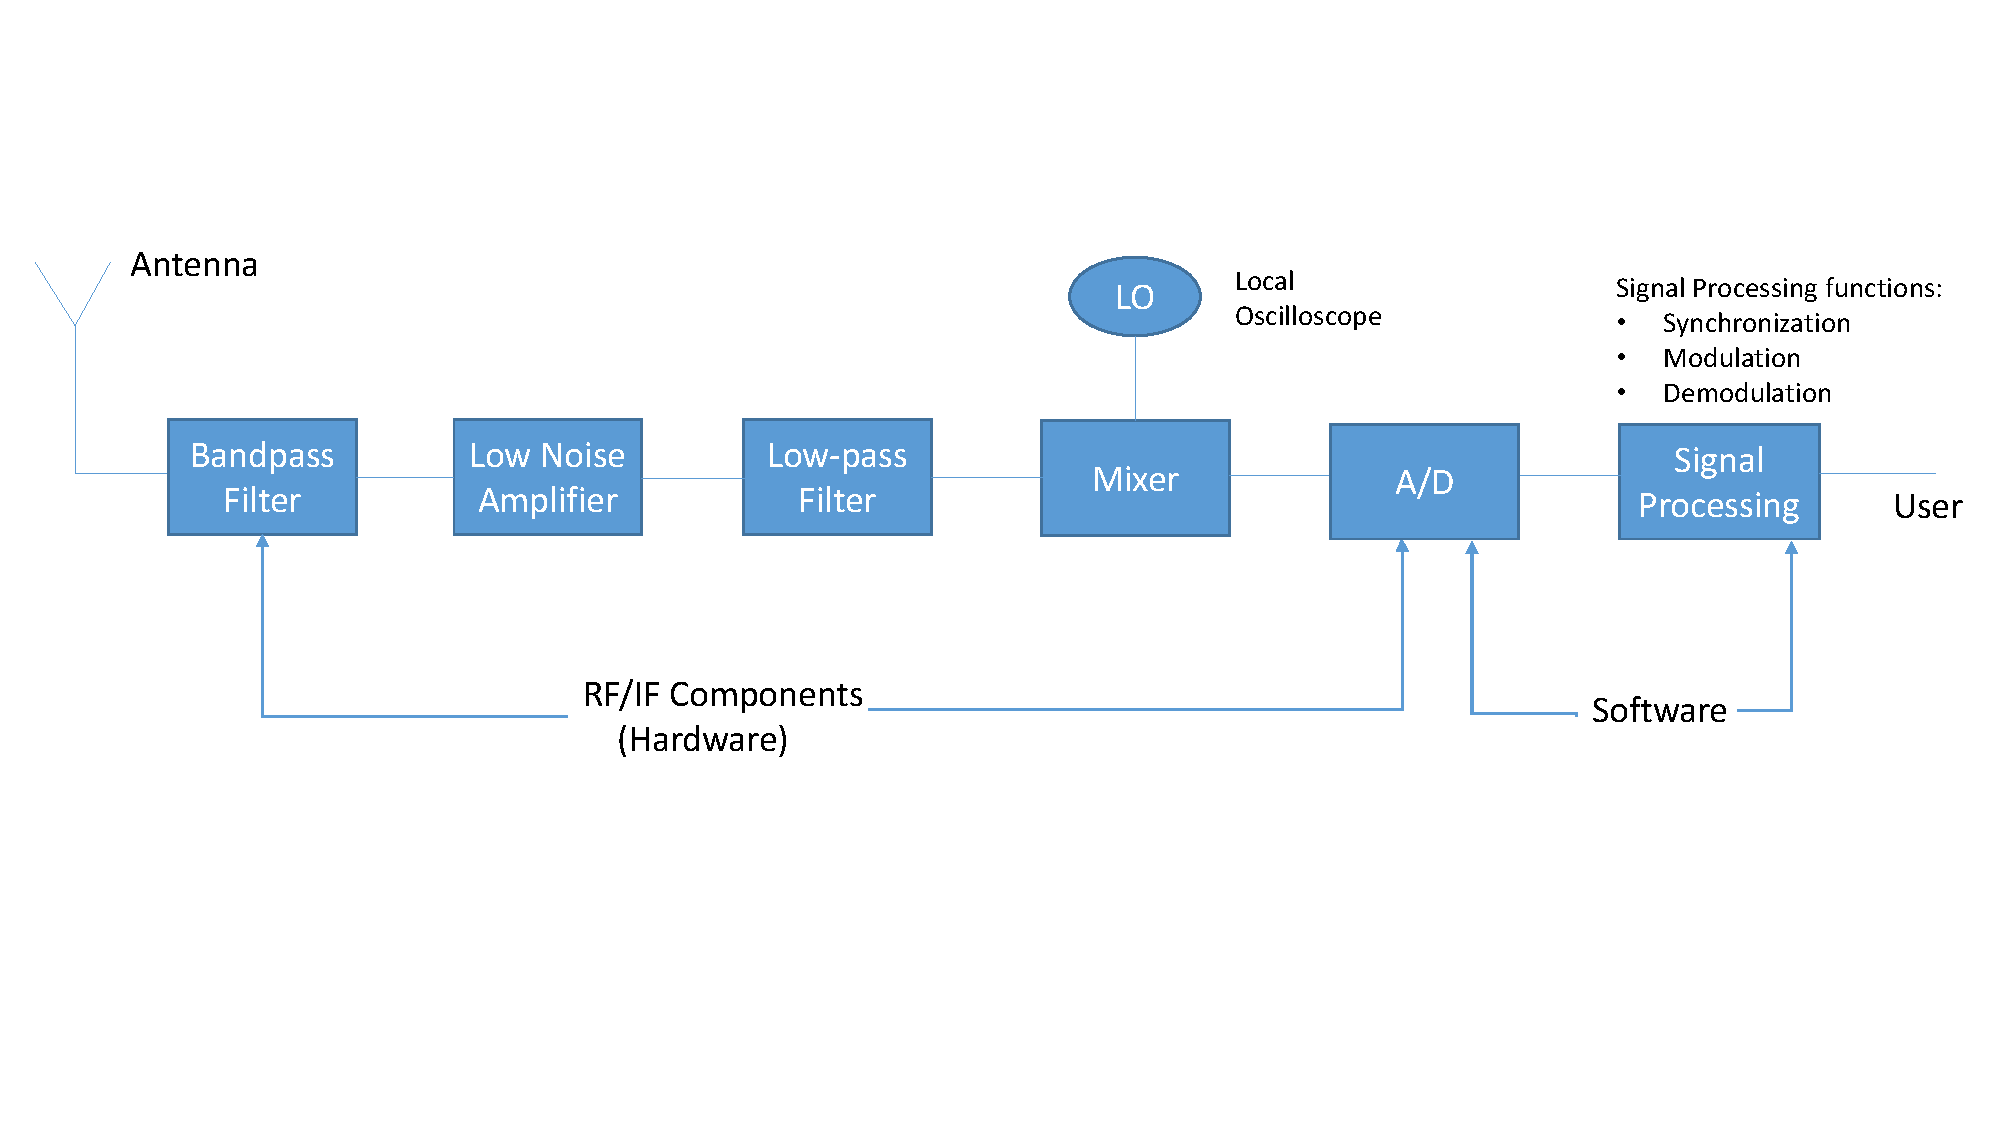
\includegraphics[width=1\textwidth]{figures/SDR.pdf}
  \caption{Components of Software Defined Radio (SDR).}
  \label{fig:SDR}
\end{figure}
\section{Software Defined Radio (SDR).}
Most of the wireless protocols in use today are implemented in hardware. With the ever increasing number of protocols to be supported and their diverse requirements, it has become apparent that a programmable environment for hardware is the need of the hour. This requirement gave rise to the concept of Software Defined Radio (SDR). SDR is a communications system in which various hardware-centric features such as filters, modulators/demodulators and other signal processing blocks are implemented in software, rather than hardware, as shown in Figure~\ref{fig:SDR}. This is a powerful concept as this design offers high flexibility and runtime reconfiguration. This methodology also has the advantage that the radio can be configured to support various physical-layer protocols based on software, eliminating the need of custom, inflexible, and expensive hardware implementations. This property of reconfigurability is an important feature for various dynamic systems utilizing cognitive radio functionalities.As a result there is a significant interest among researchers and industry alike to make SDR a reality for network operators and end users. In this thesis, we use the programmable feature of SDR to define new abstractions and expose interfaces so that a network of radios can be controlled using SDN principle. 

\section{GNU Radio framework.}
GNU Radio \cite{gnuradio} is a free and open-source framework that provides signal processing functionality to implement SDRs. The main constituents of the framework are basic blocks which perform distinct signal processing functions. GNU Radio provides great leverage to compose these blocks to synthesize new radio functionality on a general purpose hardware. But the framework alone is not suitable for developing applications to control a network of SDRs. This is because each block exposes its own set of interfaces which does not scale with increasing numbers of radios in the network. In this thesis, we provide uniform interfaces to control and manage these processing block abstractions, so that an application developer does not need to handle every block's unique interface characteristics.

